\section{GeoSPARQL}
\label{sec:geosparql}

Zoals eerder vermeld is GeoSPARQL één van de vele OGC standaarden. Specifieker is GeoSPARQL uitermate geschikt voor het uitvoeren van \acrshort{gis} queries, maar dit is zeker niet de enige mogelijkheid. Zoals eerder vermeld brengt GeoSPARQL een vocabulair voor de representatie van geospatiale gegevens, gebruik makend van RDF en is GeoSPARQL een uitbreiding op de SPARQL query taal. Het doel van GeoSPARQL is dan ook om geospatiale gegevens te verwerken. Voor het bekomen van een correcte implementatie van GeoSPARQL, zijn er normaliter meerdere voorwaarden waaraan de implementatie moet voldoen. De meeste van deze vereisten maken gebruik van de ``geo'', ``geof'' of ``geor'' ontologie \cite{ogcdocs}.

\subsection{Vereisten}
De vereisten zijn opgelijst in de officiële documentatie. Een samenvatting van het geheel is te vinden hieronder \cite{ogcdocs}. 
\begin{enumerate}
    \item \textbf{SPARQL}: Deze vereiste is meteen ook de belangrijkste. Deze stelt dat er een werkende implementatie van SPARQL aanwezig moet zijn. Dit betekent dat een implementatie GeoSPARQL ook alle mogelijkheden van SPARQL moet voorzien.
    \item \textbf{Klassen}: een correcte implementatie van GeoSPARQL moet de RDFS klassen ``geo: SpatialObject'', ``geo:Feature'' en ``geo:Geometry'' toestaan.
    \item \textbf{Properties}: verder moet een implementatie van GeoSPARQL ook verschillende attributen, zoals ``geo:sfContains'', ``geo:hasGeometry'' en ``geo:dimension'' naast vele andere, toestaan.
    \item \textbf{WKT}: RDFS \textit{literals} van het type ``geo:wktLiteral'' bevatten mogelijks een URI die het coördinaat stelsel van deze coördinaten beschrijft. Indien deze URI niet aanwezig is wordt er gekozen voor ``<http://www.opengis.net/def/crs/OGC/1.3/CRS84>''. Daarnaast moeten de coördinaten geïnterpreteerd worden zoals beschreven in het referentiesysteem.
    \item \textbf{GML}: naast WKT moet GML ook ondersteund worden. De implementatie moet zelf documenteren welke profielen ondersteund worden.
    \item \textbf{Functies}: Bij de implementatie van GeoSPARQL moeten meerdere functies ondersteund worden. Hierin is onderscheid gemaakt tussen topologische functies (zoals onder andere ``geof:sfContains'' en ``geof:ehContains'') en niet-topologische functies (zoals ``geof:distance'' en ``geof:union'').
    \item \textbf{Entailment}: GeoSPARQL moet dezelfde semantiek voor \textit{basic graph pattern matching} hanteren als SPARQL. Dit houdt in dat een functie als predikaat moet kunnen omgezet worden naar een query die ook functies berekent om aan een correct resultaat te komen. Hiervoor gebruikt het regels zoals onder andere ``geor:sfContains''.
\end{enumerate}

\subsection{Architectuur}
\label{subsec:geosparql_architecture}
\begin{figure}[ht]
    \centering
    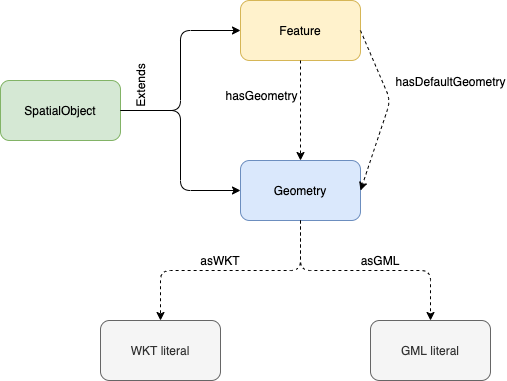
\includegraphics[width=0.5\linewidth]{images/geosparql_architecture.png}
    \caption{Vereenvoudigd diagram van de GeoSPARQL klassen ``Feature'' en ``Geometry'' met sommige properties (figuur gebaseerd op \cite{geosparqlsupport}).}
    \label{fig:geosparql_architecture}
\end{figure}

Om de architectuur vereenvoudigd weer te geven kan \figureref{fig:geosparql_architecture} helpen. Hierin is te zien dat er één hoofdklasse is waar de andere van overerven, genaamd ``SpatialObject''. Het belangrijke hier is het verschil tussen een ``Feature'' en een ``Geometry''. Een ``Geometry'' is het effectieve spatiale object, dat weergegeven kan worden als WKT of als GML (zie verder in \subsectionref{subsec:geosparql_properties}). Eén van de belangrijke (en niet vanzelfsprekende) ontwerpkeuzes is het gebruik van de ``Feature'' klasse. Deze werkt als een soort wrapper klasse voor ``Geometry''. Dit is belangrijk om te weten voor verderop in \subsectionref{subsec:geosparql_rewrite_query}, maar daar zal nogmaals terug verwezen worden naar deze subsectie.

\subsection{Properties}
\label{subsec:geosparql_properties}
GeoSPARQL voorzien een hele lijst met properties die voorzien moet worden. Vanwege de eerder korte periode om een volledige implementatie van GeoSPARQL te maken, wordt hier minder aandacht aan gegeven. Enkele voorbeelden van deze attributen zijn de volgende \cite{ogcdocs}:

\begin{itemize}
    \item \textbf{geo:isEmpty}: dit attribuut zal ``true'' terug geven indien de geometrie geen punten bevat.
    \item \textbf{geo:isSimple}: Dit attribuut zal ``true'' geven indien de geometrie geen intersecties met zichzelf bevat. Dit kan wel uitgezonderd zijn \textit{boundary} zijn.
    \item \textbf{geo:hasSerialization}: Dit attribuut wordt gebruikt om een geometrie te connecteren met zijn text-gebaseerde serialisatie. Dit kan WKT of GML zijn, maar aangezien deze uitgebreid besproken zijn in \sectionref{sec:ogc}, wordt dit hier niet herhaald. Het kan wel nogmaals benadrukt worden dat deze \textit{literal} optioneel kan bijhouden welk topologisch referentiesysteem gebruikt wordt. Het is wel belangrijk te weten waarom deze referentiesystemen zo belangrijk zijn. Australië bijvoorbeeld, verdrijft jaarlijks wat van zijn oorspronkelijke locatie. Na een aantal jaar zou elk huis op de kaart een volledig huis verder liggen, waardoor de informatie nutteloos geworden is. GeoSPARQL lost dit op met het gebruik van de referentiesystemen.
\end{itemize}


\subsection{Topologische relaties}
\label{subsec:topologische_relaties}
Om topologische relaties te kunnen beschrijven, wordt er gebruik gemaakt van drie relatiefamilies. Deze relatiefamilies beschrijven grotendeels gelijkaardige topologische relaties, maar met licht verschillende specificaties. De drie relatiefamilies zijn ``Simple Features (sf)'', ``Egenhofer (eh)'' en ``RCC8''. Om de spatiale relaties te beschrijven wordt gebruik gemaakt van een ``DE-9IM'' patroon. Voordat de relatiefamilies uitgelegd kunnen worden, is een volledig begrip van de DE-9IM notatie noodzakelijk.

\subsubsection{DE-9IM}
\begin{figure}[ht]
    \centering
    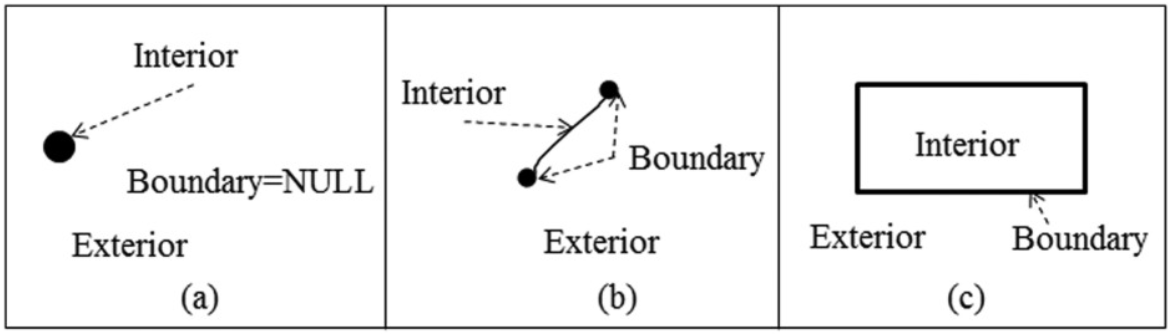
\includegraphics[width=0.9\linewidth]{images/spatial_objects_DE-9IM.png}
    \caption{Spatiale objecten met hun \textit{interior}, \textit{boundary} en \textit{exterior}: (a) Een punt; (b) Een lijn; (c) Een vlak. Figuur van \cite{shen2018classification}}.
    \label{fig:de-9im}
\end{figure}

DE-9IM staat voor \textit{Dimensionally Extended Nine-Intersection Model}. Dit model kan afgebeeld worden als een 3x3 matrix, waarbij (in deze volgorde) de \textit{interior}, \textit{boundary} en \textit{exterior} van het ene spatiale object vergeleken wordt met deze van het andere spatiale object. Deze matrix geeft de dimensies van de intersectie van deze objecten weer. De betekenis van \textit{interior}, \textit{boundary} en \textit{exterior} voor de verschillende soorten spatiale objecten is verduidelijkt in \figureref{fig:de-9im}. De volledige 3x3 matrix voor de objecten a en b is van de volgende vorm \cite{shen2018classification}:

\begin{equation*}
    DE-9IM(a,b) = 
    \begin{bmatrix}
    dim(I(a)\cap I(b)) & dim(I(a)\cap B(b)) & dim(I(a)\cap E(b))\\
    dim(B(a)\cap I(b)) & dim(B(a)\cap B(b)) & dim(B(a)\cap E(b))\\
    dim(E(a)\cap I(b)) & dim(E(a)\cap B(b)) & dim(E(a)\cap E(b))
    \end{bmatrix}
\end{equation*}

\begin{figure}[ht]
    \centering
    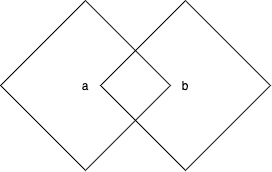
\includegraphics[width=0.5\linewidth]{images/de-9im_example.png}
    \caption{Voorbeeld voor de DE-9IM matrix.}
    \label{fig:de-9im_example}
\end{figure}

Wanneer dit toegepast wordt op de objecten die te zien zijn in \figureref{fig:de-9im_example}, dan wordt de volgende matrix bekomen:

\begin{equation*}
    DE9IM(a,b) = 
    \begin{bmatrix}
    2 & 1 & 2\\
    1 & 0 & 1\\
    2 & 1 & 2
    \end{bmatrix}
\end{equation*}

Voor het bepalen van de relaties van de GeoSPARQL families zijn er echter nog iets andere regels opgesteld. Hier heeft het OGC nieuwe betekenissen geïntroduceerd: 
\begin{enumerate}
    \item \textbf{Empty}: dit wordt genoteerd als -1.
    \item \textbf{True}: Dit geldt wanneer de waarden 0, 1, 2 voorkomen. Bij deze waarde kan soms gespecifieerd worden dat het een bepaalde waarde exact moet uitkomen. Het kan ook genoteerd worden als ``T'' (dit is trouwens meer wel dan niet het geval).
    \item \textbf{False}: dit geldt wanneer de waarde -1 wordt uitgekomen, maar wordt genoteerd als ``F''.
    \item \textbf{Don't care}: Dit betekent dat eender welke waarde mag voorkomen en dat dit hier niet naar gekeken moet worden. Dit wordt genoteerd als ``*''.
\end{enumerate}
Hierbij wordt het patroon geschreven als een sequentie van negen karakters. Als deze van links naar rechts gelezen wordt, dan stelt dit de DE-9IM matrix voor van linksboven beginnend, rij per rij opvullend. Het volgende patroon staat dus voor de overeenkomstige matrix:

\begin{equation*}
    T**T**T** = 
    \begin{bmatrix}
    T & * & *\\
    T & * & *\\
    T & * & *
    \end{bmatrix}
\end{equation*}
Indien er meer dan één lijn staat, wil dit zeggen dat één van de mogelijke matrices voldoende is om te besluiten dat de relatie klopt.

Ten slotte kunnen ook niet alle relaties voorkomen bij elke object-combinatie (bijvoorbeeld twee punten kunnen elkaar niet kruisen). Daarom wordt er ook een nieuwe notatie toegevoegd in de GeoSPARQL-documentatie, om te vermelden op welke spatiale objecten het DE-9IM intersectie patroon van toepassing is. Hierbij staat symbool ``P'' voor 0-dimensionale geometrieën (zoals punten). Het symbool ``L'' staat dan weer voor 1-dimensionale geometrieën (zoals lijnen). Het laatste symbool is ``A'', wat dan weer staat voor 2-dimensionale geometrieën (zoals vlakken) \cite{ogcdocs}.


\subsubsection{Simple Features}
\label{subsubsec:simple_features}
De eerste relatiefamilie is de ``Simple Feature'' family. De regels van deze familie worden weergegeven in \tableref{tab:topo_sf}. Hierin is exact te zien hoe de implementaties verwacht worden te werken. Om de grootte van deze masterproef in te perken is enkel deze relatiefamilie uitgewerkt en wordt dus ook enkel deze relatiefamilie besproken. Indien het voorbeeld van de ``contains'' functie besproken wordt, moet dit als volgt geïnterpreteerd worden: ``a contains b is waar, indien de intersectie van hun \textit{interiors} bestaat en hierbovenop de intersectie van de \textit{exterior} van a met zowel de \textit{interior} als de \textit{boundary} van b niet bestaat''. Dit betekent dus dat b in a ligt en dat geen enkel deel van b buiten a ligt \cite{ogcdocs}.


\begin{table}[ht]
    \centering
    \begin{tabular}{ |p{1.5cm}|l|l|p{2cm}|p{2.5cm}| } 
        \hline
        \rowcolor{TableHeaderColor} Relation Name & Relation URI & Domain/Range & Applies To Geometry Types & DE-9IM Intersection pattern \\ \hline
        
        \rowcolor{TableColor} equals & geo:sfEquals & geo:SpatialObject & All & (TFFFTFFFT) \\ \hline
        
        \rowcolor{TableColor} disjoint & geo:sfDisjoint & geo:SpatialObject & All & (FF*FF****) \\ \hline
        
        \rowcolor{TableColor} intersects & geo:sfIntersects & geo:SpatialObject & All & (T********
        *T*******
        ***T*****
        ****T****)  \\ \hline
        
        \rowcolor{TableColor} touches & geo:sfTouches & geo:SpatialObject & All except P/P & (FT*******
        F**T*****
        F***T****) \\ \hline
        
        \rowcolor{TableColor} within & geo:sfWithin & geo:SpatialObject & All & (T*F**F***) \\ \hline
        
        \rowcolor{TableColor} contains & geo:sfContains & geo:SpatialObject & All & (T*****FF*) \\ \hline
        
        \rowcolor{TableColor} overlaps & geo:sfOverlaps & geo:SpatialObject & A/A, P/P, L/L & ((T*T***T**)
        for A/A, P/P;
        (1*T***T**)
        for L/L) \\ \hline
        
        \rowcolor{TableColor} crosses & geo:sfCrosses & geo:SpatialObject & P/L, P/A, L/A, L/L & ((T*T***T**)
        for P/L, P/A,
         L/A;
        (0********)
        for L/L) \\ \hline
        
    \end{tabular}
    \caption{Simple Features Topological Relations (tabel van \cite{ogcdocs}).}
    \label{tab:topo_sf}
\end{table}


\subsection{Niet-topologische relaties}

Verder zijn er ook de niet-topologische relaties. Verschillende van deze functies gebruiken een meeteenheid URI. Daarom heeft het OGC enkele standaard meeteenheden gedefinieerd, te vinden onder de \textit{namespace} ``http://www.opengis.net/def/uom/OGC/''. Een voorbeeld van zo een meeteenheid is ``<http://www.opengis.net/def/uom/OGC/metre>''. Enkele van de niet-topologische functies zijn de volgende: \cite{ogcdocs}.

\begin{itemize}
    \item \textbf{geof:distance}: deze functie moet de kortst mogelijke afstand geven tussen twee objecten.
    \item \textbf{geof:buffer}: deze functie geeft een geometrie terug die alle punten bevat die binnen een bepaalde radius van een meegegeven geometrie liggen.
    \item \textbf{geof:convexHull}: deze functie geeft een geometrie terug die het kleinste convexe omhulsel is dat alle punten omvat van een meegegeven geometrie.
    \item \textbf{geof:intersection}: deze functie geeft een geometrie terug die staat voor alle punten van de intersectie tussen twee geometrieën.
    \item \textbf{geof:union}: deze functie geeft een geometrie terug die staat voor alle punten in de unie van twee geometrieën.
    \item \textbf{geof:envelope}: Deze functie geeft de minimaal omvattende (\textit{bounding}) \textit{box} weer voor een geometrische figuur. Dit betekent dus de kleinst mogelijke rechthoek waar elk punt van de geometrie in zit.
    
\end{itemize}

Ten slotte is het belangrijk te vermelden dat alle berekeningen horen te gebeuren in het referentiesysteem van de eerste geometrie die meegegeven is aan een functie, zowel bij topologische als niet-topologische functies \cite{ogcdocs}.


\subsection{Query Rewrite Extension}
\label{subsec:geosparql_rewrite_query}
De laatste uitdaging is het probleem waar de topologische functies als predikaat staan. Hierbij zou verwacht worden dat deze op voorhand berekend zijn en zo opgeslagen zijn in de RDF dataset. Hierbij is echter het probleem dat wanneer dit niet op voorhand berekend is, men nog steeds de correcte oplossing wil. Wanneer een deel van de gegevens uit de ene dataset komt en het andere deel uit een andere bron, zelfs dan wordt een correct antwoord verwacht, hoewel hier geen optie is tot het op voorhand uitrekenen \cite{ogcdocs}. 

Hiervoor wordt gebruik gemaakt van de \textit{query rewrite} uitbreiding. Deze techniek zal de query uitbreiden, door de unie (de SPARQL \textit{union}, niet de niet-topologische functie van GeoSPARQL!) te nemen van de oorspronkelijke stelling met enerzijds de relatie als predikaat en anderzijds het nieuwe uitgebreide deel waarbij dezelfde relatie uitgerekend wordt als functie. Hierbij is het ook belangrijk rekening te houden met het verschil tussen een ``Feature'' en een ``Geometry'' (zoals uitgelegd in \subsectionref{subsec:geosparql_architecture}), waardoor er vier extra delen nodig zijn voor de mogelijke combinaties tussen ``Feature'' en ``Geometry'' \cite{ogcdocs}. 

Zo heeft het OGC een template gemaakt om dit te herschrijven. Bij deze template zijn er een aantal placeholders gebruikt \cite{ogcdocs}:
\begin{itemize}
    \item \textbf{ogc:relation}: deze placeholder staat voor de relatie die gebruikt wordt (dit zou bijvoorbeeld de ``geo:sfContains'' kunnen zijn).
    \item \textbf{ogc:function}: deze placeholder staat voor de overeenkomstige functie bij de relatie die gebruikt wordt (in het voorbeeld van ``geo:sfContains'' zou de functie ``geof:sfContains'' zijn).
    \item \textbf{ogc:asGeomLiteral}: deze placeholder staat voor één van de serialisatie technieken om het object te bekomen.
\end{itemize}

Een voorbeeld voor het herschrijven van een query is te vinden in \listingref{listing:geosparql_query_to_rewrite}, maar de uiteindelijke template voor het herschrijven van de query is te vinden in \listingref{listing:geosparql_rewrite_query}.

\begin{listing}[ht]
    \begin{minted}{sparql}
        select *
        where {
            { ?f1 ogc:relation ?f2 . }
        }
    \end{minted}
    \caption{Query to rewrite.}
    \label{listing:geosparql_query_to_rewrite}
\end{listing}

\begin{listing}[ht]
    \begin{minted}{sparql}
        select *
        where {
            { ?f1 ogc:relation ?f2 . }
            UNION
            # feature - feature rule
            {   ?f1 geo:hasDefaultGeometry ?g1 . 
                ?f2 geo:hasDefaultGeometry ?g2 .
                ?g1 ogc:asGeomLiteral ?g1Serial .
                ?g2 ogc:asGeomLiteral ?g2Serial .
                filter(ogc:function(?g1Serial, ?g2Serial)) }
            UNION
            # feature - geometry rule
            {   ?f1 geo:hasDefaultGeometry ?g1 . 
                ?g1 ogc:asGeomLiteral ?g1Serial .
                ?f2 ogc:asGeomLiteral ?g2Serial .
                filter(ogc:function(?g1Serial, ?g2Serial)) }
            UNION
            # geometry - feature rule
            {   ?f2 geo:hasDefaultGeometry ?g2 .
                ?f1 ogc:asGeomLiteral ?g1Serial .
                ?g2 ogc:asGeomLiteral ?g2Serial .
                filter(ogc:function(?g1Serial, ?g2Serial)) }
            UNION
            # geometry - geometry rule
            {   ?f1 ogc:asGeomLiteral ?g1Serial .
                ?f2 ogc:asGeomLiteral ?g2Serial .
                filter(ogc:function(?g1Serial, ?g2Serial)) }
        }
    \end{minted}
    \caption{Query rewrite template (listing van \cite{ogcdocs}).}
    \label{listing:geosparql_rewrite_query}
\end{listing}